\documentclass[8pt,letterpaper]{book}
\usepackage{fullpage}
\usepackage[top=2cm, bottom=4.5cm, left=2cm, right=2cm]{geometry}
\usepackage{amsmath,amsthm,amsfonts,amssymb,amscd}
\usepackage{lastpage}
\usepackage{enumerate}
\usepackage{fancyhdr}
\usepackage{mathrsfs}
\usepackage{xcolor}
\usepackage{graphicx}
\usepackage{listings}
\usepackage{hyperref}
\usepackage{mdframed}
\usepackage{changepage}   % for the adjustwidth environment
\usepackage{forest} 
\usepackage{tikz}   % For graph

\usepackage[english]{babel}
\usepackage[utf8]{inputenc}
\usepackage{float}

\pagestyle{headings}
% \graphicspath{{../}}

\hypersetup{%
  colorlinks=true,
  linkcolor=blue,
  linkbordercolor={0 0 1}
}
\newcommand\mkbibcolor[2]{\textcolor{blue}{\hypersetup{citecolor=#1}#2}}

\setlength{\parindent}{0.0in}
\setlength{\parskip}{0.05in}

\newcommand\projnumber{1}
\newcommand\course{CS 575}
\newcommand\OSUID{934370552}
\newcommand\Email{buivy@oregonstate.edu}
\newcommand\Name{Vy Bui}
\newcommand\tab[1][1cm]{\hspace*{#1}}

\pagestyle{fancyplain}
\headheight 35pt
% \lhead{\textbf{Project \projnumber}}
% \rhead{April 4, 2022}
\lfoot{}
\cfoot{}
\rfoot{\small\thepage}
\headsep 1.5em

% Redefine proof end symbol
\renewcommand\qedsymbol{$\blacksquare$}

\newcommand{\Tau}{\mathrm{T}}
\newenvironment{problem}[2][Problem]
    { \begin{mdframed}[backgroundcolor=gray!20] \textbf{#1 #2} \\}
    {  \end{mdframed}}
   

% Make Rightarrow with superscript
\makeatletter
\newcommand{\xRightarrow}[2][]{\ext@arrow 0359\Rightarrowfill@{#1}{#2}}
\makeatother

\begin{document}

\begin{titlepage}
    \begin{center}
        \vspace*{4cm}

        \textbf{\Large CS534 - MACHINE LEARNING}

        \vspace{1cm}

        Author: Vy Bui
        
        Email: buivy@oregonstate.edu
 
        \vfill
             
        \vspace{0.8cm}
      
             
        The School of Electrical Engineering and Computer Science\\
        Oregon State University\\
             
    \end{center}
 \end{titlepage}

%================================= CONTENT ====================================%
\tableofcontents

\pagebreak
\chapter{SPAM PREDICTOR}
\chapter{LINEAR REGRESSION}
\chapter{LOGISTIC REGRESSION}
\chapter{FEATURE SELECTION}


\chapter{PERCEPTRON}

A perceptron is a binary classifier using the Heaviside step function instead of 
sigmoid as in Logistic Regression. Because this function is not differentiable, 
gradient descent cannot be used, and the perceptron learning algorithm is used 
instead.

\section{Algorithm Learning Algorithm}
The algorithm starts with random weights, iteratively updates them whenever the 
model makes a prediction mistake.

$$w_{t+1} = w_t - \eta_t (\hat{y}_n - y_n)x_n$$

Intuitively, if $y_n = 1$ and $\hat{y}_n = 0$, we have $w_{t+1} = w_t + x_n$, 
and if $y_n = 0$ and $\hat{y}_n = 1$, we have $w_{t+1} = w_t - x_n$.

\section{Perceptron/hinge loss}
\textbf{Perceptron loss}
$$L_P(w) = \frac{1}{N} \sum_{i=1}^{N} max(0,-y_i \mathbf{w}^T \mathbf{x}_i)$$

\begin{figure}[H]
    \centering
    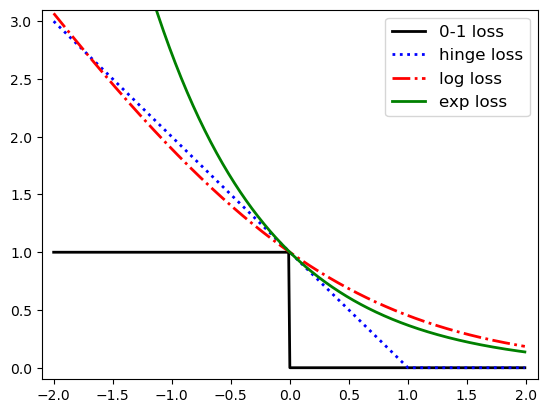
\includegraphics[scale=0.5]{losses.png} \par
    \caption{Various loss functions}
    \label{loss_functions}
\end{figure}

\section{Sub-gradient descent}
The Subgradients of a convex function is a way of generalizing the notion of a 
derivative to work with functions which have local discontinuities. For a convex 
function of several variables, $f : R^n \rightarrow R^n$, we say that 
$g \in R^n$ is a \textbf{subgradient} of $f$ at $\mathbf{x} \in dom(f)$ if for 
all vectors $z \in dom(f)$

$$f(z) \geq f(\mathbf{x}) + \mathbf{g}^T (\mathbf{z - x})$$

\begin{figure}[H]
    \centering
    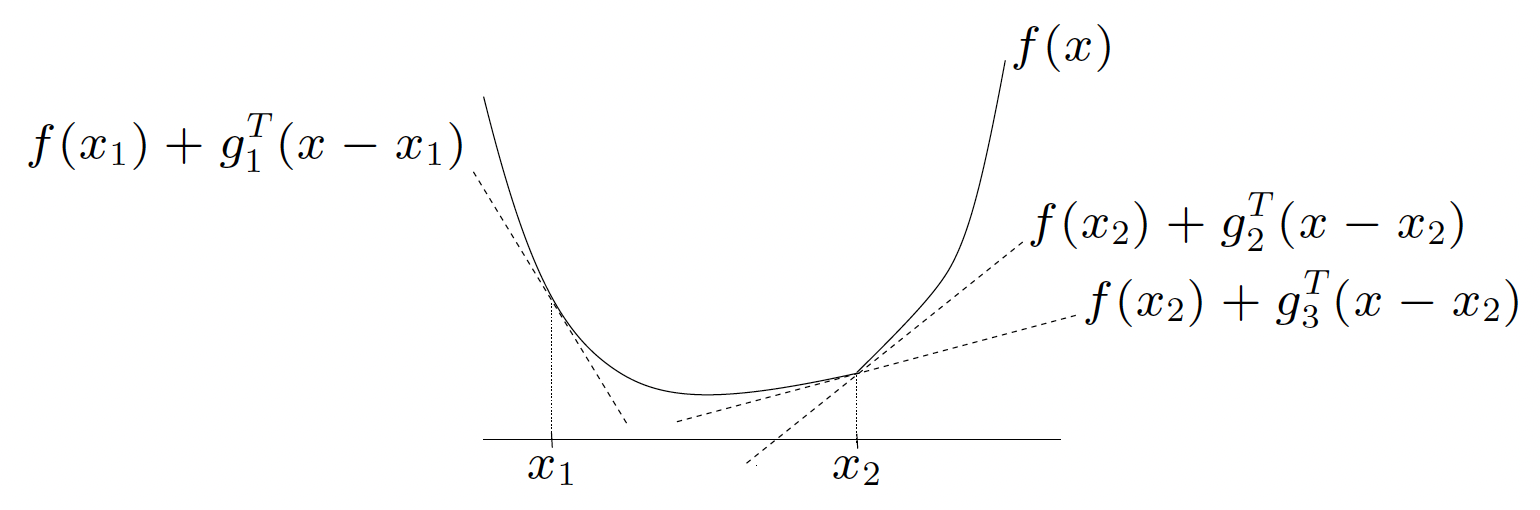
\includegraphics[scale=0.5]{subgradients.png} \par
    \caption{Illustration of subgradients}
    \label{subgradient_illustration}
\end{figure}

\section{Perceptron Convergence Theorem}
If data is \textbf{linearly separable}, perceptron algorithm will find a linear 
classifier that classifies all data correctly in at most $O(r^2 / \gamma^2)$, 
where $r = max||X_i||$ is \textbf{the radius of data} and $\gamma$ is the 
\textbf{maximum margin}.

\textbf{Margin} is the min distance from data points to the decision boundary. 
The bigger the margin is, the easier the classification problem is. Also, the 
model will converge faster.

\section{}
\section{}



Voted and Average Perceptrons
Structured Perceptrons



\chapter{KERNEL METHODS}
By definition, kernels are functions 
$k : X \times X \rightarrow \mathbb{R}$ for which there exists a Hilbert space 
$\mathbb{H}$ and a feature map $\phi : X \rightarrow \mathbb{H}$ such that

$$
k(x,x') = \phi(x)^T \phi(x')
$$

Intuitively speaking, kernels calculate the relationships between every pair of 
observations. And these observations are used to find the 
\textbf{support vector classifier}. 

\textbf{The kernel trick} helps calculate the relationships between every pair 
as if they are in the higher dimensions but they actually don't do the 
transformation. This reduces the amount of computation significantly.

Inner product?
Hilbert space?

Design matrix $\Phi$

dual representation

Gram matrix $K = \Phi \Phi^T$

positive semidefinite matrix

\chapter{SVM}
SVM?

Linear SVM?

Non-linear SVM?

\textbf{Hard/Maximum margin SVM issues} \newline
- Has no solution for nonlinearly separable data \newline
- Overfits to outliers \newline

\textbf{Soft margin} \newline
- Introduce slack to the hard margin constraints (allow misclassification, 
bias/variance tradeoff) \newline
- Minimizing L2 Regularized \newline
- Data points for which $\epsilon = 0$ are correctly classified 
and are either on the margin or on the correct side of the margin. Points for which 
$0 < \epsilon \leq 1$ lie inside the margin, but on the correct side of the 
decision boundary, and those data points for which $\epsilon > 1$ lie on
the wrong side of the decision boundary and are misclassified.
- Support Vectors include Margin Support Vectors ($\epsilon = 0$) and 
Non-margin Support Vectors ($\epsilon > 0$ and $0 < \epsilon < 1$ and $\epsilon > 1$)

$L_2$ SVM?



%================================= CHAPTER ====================================%
%================================= SECTION ====================================%
\chapter{NAIVE BAYES}

%================================= CHAPTER ====================================%
\chapter{DECISION TREE}
%================================= SECTION ====================================%
\section{Mutual Information}
\textbf{Entropy}
\begin{equation}\label{eqn:entropy}
    H(X) = -\sum_{k=1}^{K} p(X=k) log_2 p(X=k)
\end{equation}

\textbf{Entropy for Binary Random Variable}
\begin{equation}\label{eqn:binary_entropy}
    H(X) = -p(X=1)log_2 p(X=1) - p(X=0)log_2 p(X=0)
\end{equation}


\textbf{Joint Entropy}
\begin{equation}\label{eqn:joint_entropy}
    H(X,Y) = -\sum_{x,y} p(x,y) log_2 p(x,y)
\end{equation}

\textbf{Conditional Entropy}

\begin{equation}\label{eqn:cond_entropy}
    H(Y|X) = H(X,Y) - H(X)
    = -\sum_{x,y} p(x,y) log_2 p(x,y) -\sum_{x} p(x) log_2 \frac{1}{p(x)}
\end{equation}

or more general

\begin{equation}\label{eqn:cond_entropy_general}
    H((X_1,X_2,...,X_n)) = \sum_{i=1}^{n} H(X_i | X_1,...,X_{i-1})
\end{equation}

\eqref{eqn:cond_entropy}

Mutual information tells us how similar two distributions are.

\begin{equation}\label{eqn:mutual_information}
    I(X,Y) = H(X) - H(X|Y) = H(Y) - H(Y|X)
\end{equation}

\cite{Murphy22}, 6.3 \newline

Notes from \cite{Murphy22}, 18 \newline
\begin{itemize}
    \item Multi-way split might cause \textbf{data fragmentation} (too little data might fall into each subtree), resulting in overfitting.
    \item 
    \item 
\end{itemize}


\cite{HasTibFri17}, 9.2 \newline

%================================= CHAPTER ====================================%
\chapter{Emsemble Methods}
%================================= SECTION ====================================%
\section{Bagging}
refer to \cite{Murphy22}, chapter 18.3 Bagging. \newline
%================================= SECTION ====================================%
\section{Boosting}
\cite{Bishop06}, 14.3 \newline

%================================= CHAPTER ====================================%
%================================= SECTION ====================================%
\chapter{Unsupervised Learning}
\section{Clustering}
For \textbf{Hierarchical Clustering}, refer to \cite{Murphy22}, chapter 21.2 Hierarchical clustering. \newline

For \textbf{Flat Clustering}, refer to \cite{Murphy22}, chapter 21.3 K Means Clustering. \newline


%==============================================================================%
\chapter{Dimensionality Reduction}

%------------------------------------------------------------------------------%
\section{Motivation}
Many problems involve a huge number of features, which make the training more expensive and make it harder to search for a good solution. This problem is known as the \textit{curse of dimensionality}. Oftentimes, reducing the number of features can 

\begin{itemize}
    \item speed up training
    \item filter out noise and unnecessary details, thus result in higher performance models.
    \item useful for data visualization
\end{itemize}

Furthermore, in high-dimensional data sets, data points are likely to be far from each other (sparse), and new data point will also be far from training data points, which makes prediction less reliable than in lower dimensions. In other words, models trained on higher dimension data sets are prone to overfitting \cite{Geron19}.

%------------------------------------------------------------------------------%
\section{Prerequisite}
Linear Algebra: Eigenvectors
Statistics: covariance

%------------------------------------------------------------------------------%
\section{Approaches}
There are two main approaches to reducing dimensionality: Projection and Manifold Learning.

\subsection{Projection}

\subsection{Manifold Learning}






%================================= CHAPTER ====================================%
\bibliographystyle{alpha}
\bibliography{mybib}

\end{document}

